%++++++++++++++++++++++++++++++++++++++++
% Don't modify this section unless you know what you're doing!
\documentclass[
letterpaper,
12pt,
singlespacing,
headsepline]{article}

\usepackage{tabularx} % extra features for tabular environment
\usepackage{amsmath}  % improve math presentation
\usepackage{graphicx} % takes care of graphic including machinery
\usepackage[margin=1in,letterpaper]{geometry} % decreases margins
\usepackage[final]{hyperref} % adds hyper links inside the generated pdf file
\usepackage[utf8]{inputenc} % Required for inputting international characters
\usepackage[T1]{fontenc} % Output font encoding for international characters
\usepackage[spanish]{babel}
\usepackage{mathpazo} % Use the Palatino font by default

\usepackage[backend=bibtex,style=authoryear,natbib=true]{biblatex} % Use the bibtex backend with the authoryear citation style (which resembles APA)

\addbibresource{references/references1.bib} % The filename of the bibliography

\usepackage[autostyle=true]{csquotes} % Required to generate language-dependent quotes in the bibliography
\hypersetup{
	colorlinks=true,       % false: boxed links; true: colored links
	linkcolor=blue,        % color of internal links
	citecolor=blue,        % color of links to bibliography
	filecolor=magenta,     % color of file links
	urlcolor=blue         
}
%++++++++++++++++++++++++++++++++++++++++


\begin{document}
	\begin{titlepage}
	\vspace*{\stretch{0.5}}
	   \begin{center}
			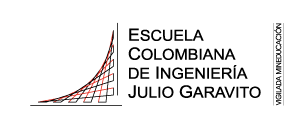
\includegraphics[scale=0.5]{Images/1110_logotipo_institucional_vm300px.png} \\
		    \Large{\textbf{Escuela Colombiana de Ingeniería Julio Garavito}\vspace{2cm}}\\
		    \textbf{Maestría en Gestión de Información}\vspace{1cm}\\
		    \textbf{Ley en Gestión de Información}\vspace{1cm}\\
			\textsc{Taller 1} \vspace{2cm}  \\   
			\emph{Autor:} \textit{Ing. Fabio Quintero}\vspace{5cm}\\
	     \textit{\today}\\

	   \end{center}
	   \vspace*{\stretch{2.0}}
	\end{titlepage}
	






\section{Derechos de Autor}

\subsection{Participación ciudadana}


\subsection{Participación como opción de grado}


\section{Protección de datos}
\subsection{Datos públicos vs datos interés público}
\subsection{Datos semiprivados}



\section{Analysis}

In this section you will need to show your experimental results. Use tables and
graphs when it is possible. Table~\ref{tbl:bins} is an example.

\begin{table}[ht]
\begin{center}
\caption{Every table needs a caption.}
\label{tbl:bins} % spaces are big no-no withing labels
\begin{tabular}{|cc|} 
\hline
\multicolumn{1}{|c}{$x$ (m)} & \multicolumn{1}{c|}{$V$ (V)} \\
\hline
0.0044151 &   0.0030871 \\
0.0021633 &   0.0021343 \\
0.0003600 &   0.0018642 \\
0.0023831 &   0.0013287 \\
\hline
\end{tabular}
\end{center}
\end{table}

Analysis of equation~\ref{eq:aperp} shows ...

Note: this section can be integrated with the previous one as long as you
address the issue. Here explain how you determine uncertainties for different
measured values. Suppose that in the experiment you make a series of
measurements of a resistance of the wire $R$ for different applied voltages
$V$, then you calculate the temperature from the resistance using a known
equation and make a plot  temperature vs. voltage squared. Again suppose that
this dependence is expected to be linear~\cite{Cyr}, and the proportionality coefficient
is extracted from the graph. Then what you need to explain is that for the
resistance and the voltage the uncertainties are instrumental (since each
measurements in done only once), and they are $\dots$. Then give an equation
for calculating the uncertainty of the temperature from the resistance
uncertainty. Finally explain how the uncertainty of the slop of the graph was
found (computer fitting, graphical method, \emph{etc}.)

If in the process of data analysis you found any noticeable systematic
error(s), you have to explain them in this section of the report.

It is also recommended to plot the data graphically to efficiently illustrate
any points of discussion. For example, it is easy to conclude that the
experiment and theory match each other rather well if you look at
Fig.~\ref{fig:samplesetup} and Fig.~\ref{fig:exp_plots}.

%\begin{figure}[ht] 
%  \centering
%      \includegraphics[width=0.5\columnwidth]{sr_squeezing_vs_detuning}

% some figures do not need to be too wide
%        \caption{
%                \label{fig:exp_plots}  
%                Every plot must have axes labeled.
%        }
%\end{figure}


\section{Conclusions}
Here you briefly summarize your findings.



%----------------------------------------------------------------------------------------
%	BIBLIOGRAPHY
%----------------------------------------------------------------------------------------

\printbibliography[heading=bibintoc]


\end{document}
